\documentclass{article}
\usepackage{graphicx} % Required for inserting images
\usepackage{float}
\usepackage{geometry}
\geometry{left=1in, right=1in, top=1in, bottom=1in}

\title{\Huge Software Requirements Specifications \\for Snakes and Ladders CS261 OOPS Project}

\date{18 October 2023}
\author{Yuvraj, Shreyas, Sneha, Suraj}

\begin{document}

\maketitle

\section{Introduction}
    \begin{itemize}
        \item The Snakes and Ladders Game is a digital recreation of the classic board game. The primary aim is to provide an enjoyable and interactive gaming experience for players of all ages.
        \item In the project we implement all the concepts of Object Oriented Analysis and Design as well as Object oriented Programming to achieve the goal of creating this semester Project.
        \item We aim to achieve this by using a Web Application interface in order to have a seem less experience of using our product. Due to the simplistic nature of the design this project can be replicated or used by any person even with limited compute power as it will not be hardware heavy.
    \end{itemize}

\section{Objective for the Project}
    \begin{itemize}
        \item The major objective of this project is to prove that Object oriented approach to a relatively complex problem can help in breaking down the problem and provide a better solution to our project.
        \item Another goal for this project is to show that how processes like abstraction and inheritance can help in designing the product much more efficiently.
        \item Using Object oriented concepts can also help in reducing the debugging time frame and provides a better CI/CD Pipeline for the product.
        \item By utilizing the Web-App interface we ensure that there is no need of looking after compatibility issues like device support or any of such sort. A simple Web-App ensures that the product is playable on all devices that have a working internet browser and an active internet connection.
    \end{itemize}

\newpage

\section{Functional Requirements}
    \begin{itemize}
        \item \textbf{Die Rolling:} Implement random die roll functionality (1-6).
        \item \textbf{Player Movement:} Move the player's game piece based on the die roll.
        \item \textbf{Consecutive 6s Rule:} Detect three consecutive 6s and void the last 6.
        \item \textbf{Normal Block:} Move the player to the designated block.
        \item \textbf{Snake Head Block:} Move the player to the corresponding snake's tail block.
        \item \textbf{Ladder Bottom Block:} Move the player to the corresponding ladder's top block.
    \end{itemize}

\section{Non-Functional Requirements}
    \begin{itemize}
        \item \textbf{User Interface:} Intuitive and visually appealing user interface.
        \item \textbf{Performance:} Smooth game play with responsive controls.
        \item \textbf{Compatibility:} The game should run on popular web browsers.
        \item \textbf{Security:} Ensure data privacy and prevent cheating.
    \end{itemize}

\section{Tech Stacks Used}

    \begin{enumerate}
        \item \textbf{Front End: }
            \begin{itemize}
                \item React
                \item CSS (Tailwind)
            \end{itemize}

        \item \textbf{Back End: }
            \begin{itemize}
                \item Django
            \end{itemize}

        \item \textbf{Version Control: }
        \begin{itemize}
            \item Git
            \item GitHub
        \end{itemize}
    \end{enumerate}
\section{General Working}
    \begin{itemize}
        \item The game first starts by first giving the control to player to roll the dice where as soon as player clicks the icon of dice, by using a random number generator a number between 1 and 6 is generated.
        \item When the number is generated the computer inputs it and moves the respective piece accordingly. These two processes are repeated until one of the player reaches 100.
        \item If the player lands on a snake mouth his/her piece will travel down to its tail cell.
        \item If the player lands on a ladder's start his/her piece will travel up the ladder.
        \item First player to reach 100 will win the game.
    \end{itemize}
\section{Use Case and Class Diagram}

\begin{figure}[H]
    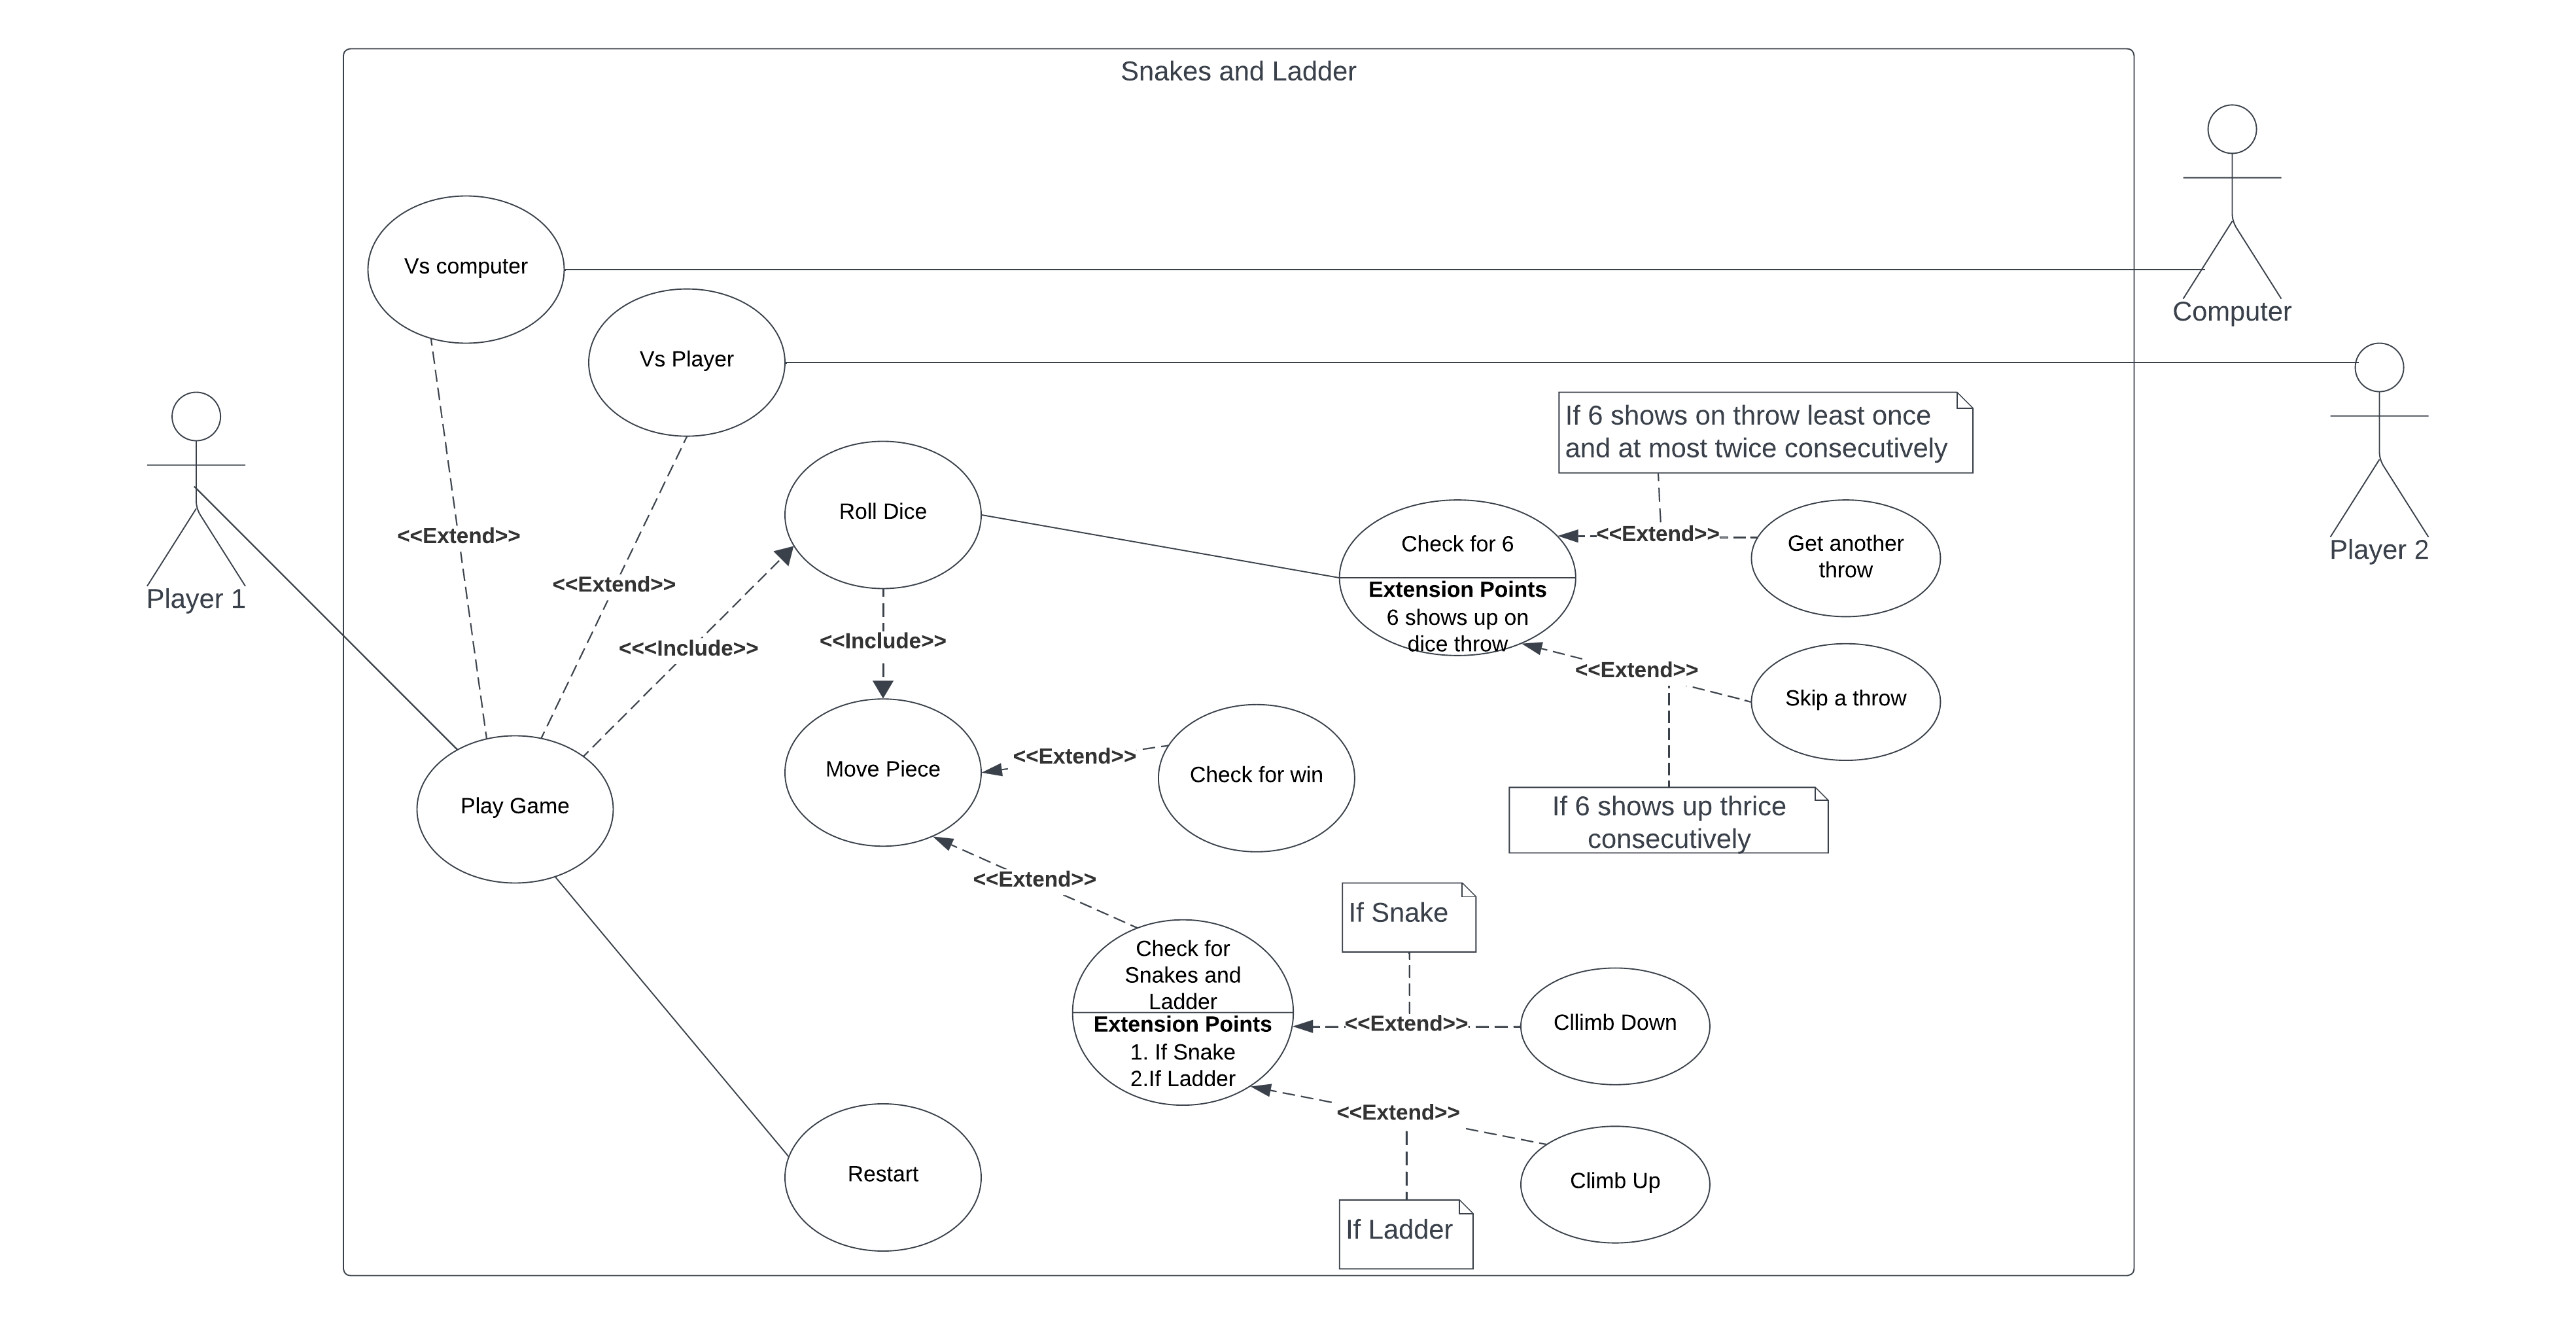
\includegraphics[width = 0.90\linewidth]{Images/Use Case Diagram.png}
    \caption{Use Case Diagram}
\end{figure}

\begin{figure}[H]
    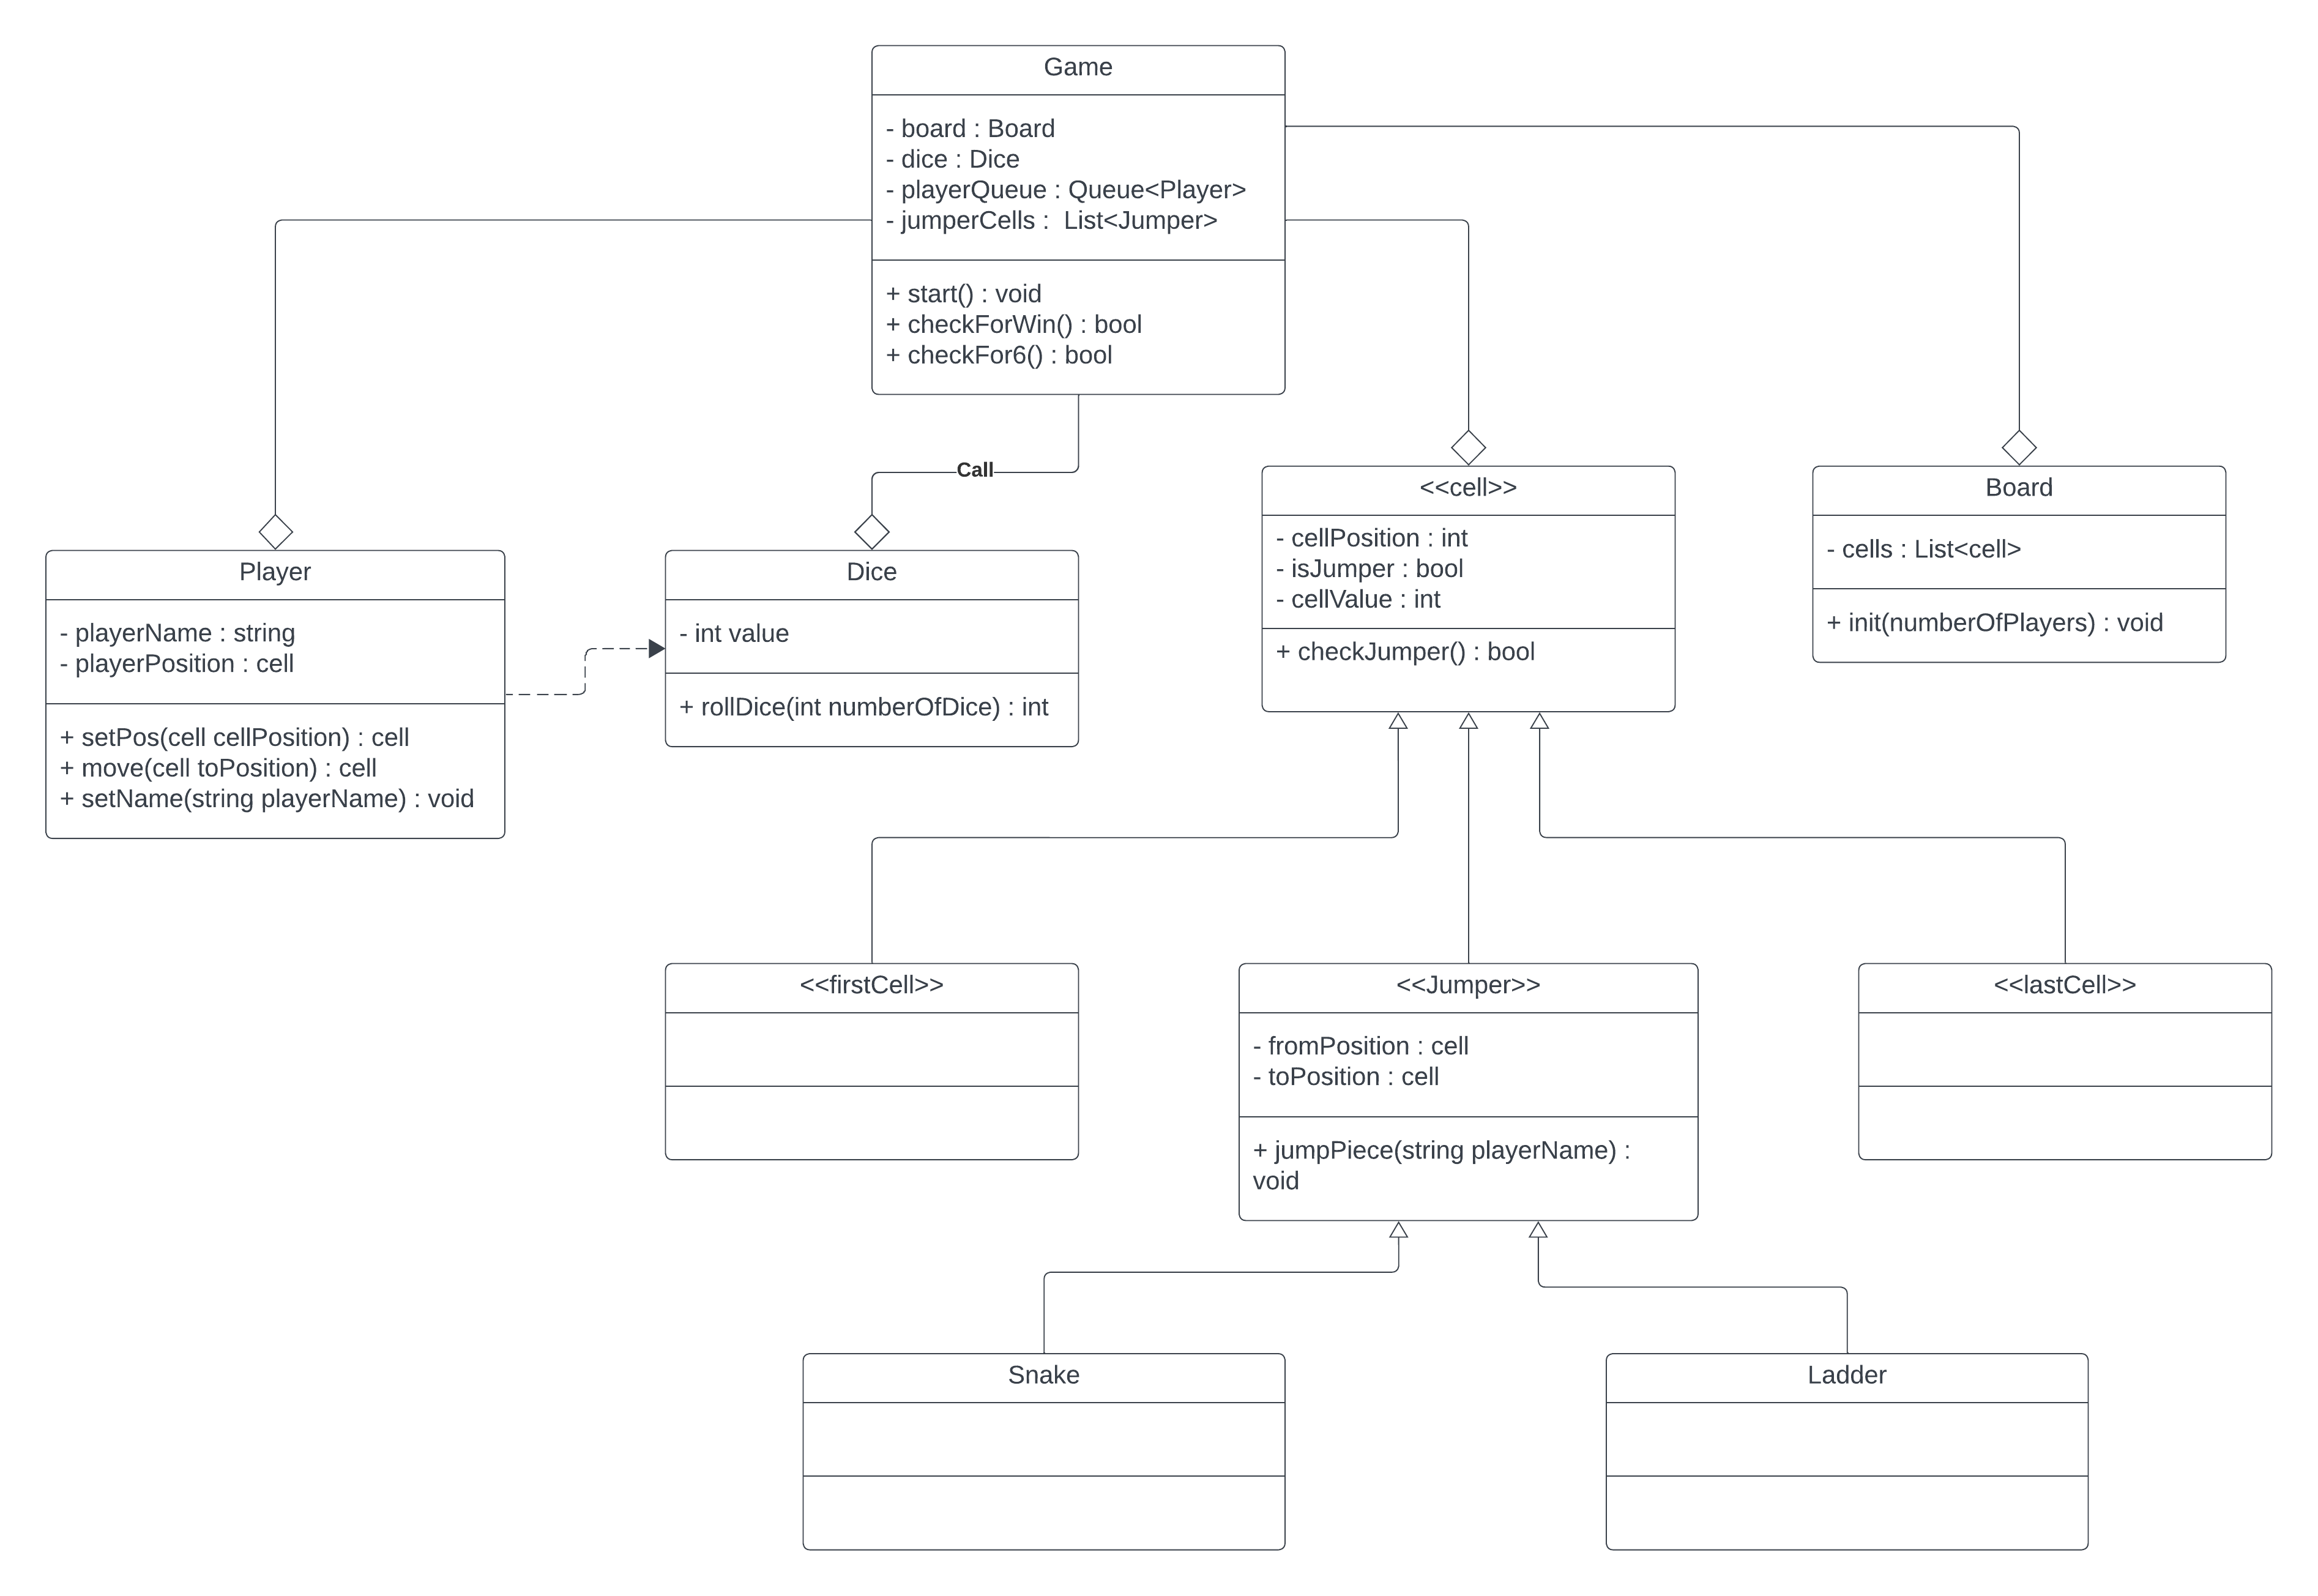
\includegraphics[width = 0.90\linewidth]{Images/Class Diagram.png}
    \caption{Class Diagram}
\end{figure}

\newpage
    
\end{document}
